% !TEX root = main.tex

\section{実験目的}

産業用ロボットの多くは,複数のリンクと回転関節から構成されるシリアルリンク型である.
本実験では,6自由度垂直多関節型のマニピュレータを用いて,
ティーチングと呼ばれる産業用ロボットのプログラムを作成する方法を学ぶ.
また,マニピュレータの制御で用いられる運動学の基礎知識を習得する.
さらに,カメラを用いた物体検知と3次元位置計測を通じて,ロボットビジョンの基礎技術を学ぶ.


\section{多自由度マニピュレータ}

\subsection{ティーチング}
マニピュレータ(産業用ロボット)の制御は,運動学や軌道決定を計算し,
モータを制御するなどのマニピュレータの動きを含めた制御に分けて考える必要がある.
前者については,4年後期の講義「ロボティクスII」にて基礎知識を学ぶ.
後者のマニピュレータへの動作入力方法には,ティーチングとよばれる表示方法が用いられている.

ティーチングは,ダイレクトティーチング,オンラインティーチング,オフラインティーチングに分類される.
ダイレクトティーチングはマニピュレータ本体に直接(ダイレクト)
に触れながらマニピュレータの動作を記録し,記録した動作をプレイバック(再現)する.
オンラインティーチングはティーチングペンダントと呼ばれるインターフェイスを使用して,
マニピュレータを手動操作し,動作を記録,プレイバックさせる.
オフラインティーチングは,コンピュータ上でシミュレータを操作し,
動作を記録する.そして,実際のマニピュレータにデータを送信し,
プレイバックさせる方法である.

\subsection{システム構成}
本実験で用いる多自由度マニピュレータは,xArm 6(UFACTORY製)である.
6個の回転関節を有するため,自由度は3次元空間の位置姿勢を任意に決めることができる6自由度である.
各関節はサーボモータによって駆動され,関節角度はアブソリュート型エンコーダによって取得される.

本実験システムは,マニピュレータ,空圧駆動型ロボットグリッパおよび制御PC,
ノートPCから構成される.図2.1にマニピュレータのシステム構成を示す.
制御PCはLinuxと呼ばれるOSが搭載されており,制御周期10msでマニピュレータを制御している.
制御PC内では,マニピュレータの運動学,姿勢,軌道の計算,モータの制御などが行われており,
マニピュレータの動きを統合的にコントロールしている.
ノートPCは専用の制御ソフトウェアを用いることで,マニピュレータの手動操作,
状態の確認やティーチング,各種設定を行うことができる.
つまり,ティーチングペンダントと同等の操作ができる.
また,Pythonを用いることで,ロボットビジョンやAIを活用したマニピュレータへの動作指示の送信や,
マニピュレータの状態を受信することも可能である.

\begin{figure}[h]
  \centering
  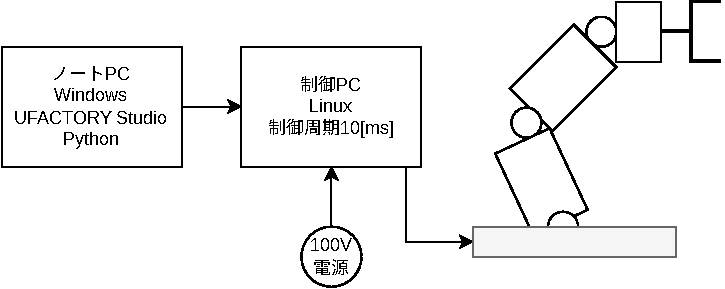
\includegraphics[scale=1]{sozai/1.pdf}
  \caption{システム構成}
\end{figure}


\subsection{マニピュレータの運動学}
各関節角度を入力として,手先の位置姿勢を求める問題を順運動学という.
一方で,手先の位置姿勢を入力として各関節角度を求める問題を逆運動学という.
本実験では,マニピュレータの第4~第6関節を固定し,
3自由度マニピュレータとして運動学を考える.
これは,マニピュレータを簡単な構造として,運動学を幾何学計算するためである.

\subsubsection{順運動学}
グローバル座標系$\Sigma_0$の原点から$z_0$軸方向に$l_1$平行移動した
座標系$\Sigma$からみた手先位置を計算する.幾何学的に考える場合,
まず$x'z'$平面で考える.三角関数を用いると,手先位置$[x' \ z']^T$は,

\begin{align}
  x' & = l_2 \cos (\varphi_1 - \theta_2) - l_3 \cos \{ (\varphi_1 - \theta_2) + (\varphi_2 - \theta_3) \} \tag{2.1} \\
  z  & = l_2 \sin (\varphi_1 - \theta_2) - l_3 \sin \{ (\varphi_1 - \theta_2) + (\varphi_2 - \theta_3) \} 
\end{align}

となる.次に,座標系$\Sigma$の原点から手先位置を$xy$平面に射影すると,
式(2.1)より大きさ$|x'|$を用いて,

\begin{align}
  x & = |x'| \cos \theta_1 \tag{2.2} \\
  y & = |x'| \sin \theta_1 
\end{align}

と計算することができる.また,グローバル座標系$\Sigma_0$からみた手先位置は,
式(2.1),式(2.2)を用いて,

\begin{align}
  \begin{bmatrix}
    x \\
    y \\
    z
  \end{bmatrix}
  = 
  \begin{bmatrix}
    x \\
    y \\
    z + l_1
  \end{bmatrix} \tag{2.3}
\end{align}

となる.

\subsubsection{逆運動学}
逆運動学について説明する.グローバル座標系からみた手先位置
$\begin{bmatrix} x_0 \ y_0 \ z_0 \end{bmatrix}^T$が既知の場合,

\begin{align}
  \begin{bmatrix} x \\ y \\ z \end{bmatrix} = \begin{bmatrix} x_0 \\ y_0 \\ z_0 - l_1 \end{bmatrix} \tag{2.4}
\end{align}

と座標系$\Sigma$からみた手先位置を求めることができる.
つまり,手先位置$[x \ y \ z]^T$が既知となった.
次に,座標系$\Sigma$の$xy$平面を考えると,関節角度$\theta_1$は,

\begin{align}
  \theta_1 = \tan^{-1} \frac{y}{x} \tag{2.5}
\end{align}

と$x, y$を用いて計算できる.なお,$x^2 + y^2 = 0$のときは,
$\theta_1$は一意に決まらず,任意の値になる.ここで,アークタンジェントは,
プログラミング言語において$\text{atan}$と$\text{atan2}$の2種類存在する.
今回は,戻り値の範囲が広い$\text{atan2}$を使用する.

\begin{align}
  \theta_1 = \text{atan2}(y, x) \tag{2.6}
\end{align}

以下,アークタンジェントは$\text{atan2}$で表記する.

次に関節角度$\theta_3$を余弦定理から求める.
先に計算に必要な$x'$について求める.
$xy$平面の原点から手先位置を射影した点までの長さは

\begin{align}
  |x'| = \sqrt{x^2 + y^2} \tag{2.7}
\end{align}

と$x, y$を用いて計算できる.絶対値を外すと,

\begin{align}
  x' = \pm \sqrt{x^2 + y^2} \tag{2.8}
\end{align}

である.この値を用いて余弦定理を適用する.
余弦定理は,三角形$ABC$に対し,辺$AB, AC$のなす角を$\theta$とすると,

\begin{align}
  BC^2 = AB^2 + AC^2 - 2 AB \cdot AC \cos \theta \tag{2.9}
\end{align}

という関係式が成立する定理である.$x'z'$平面の三角形に注目すると,
余弦定理を適用して

\begin{align}
  \cos(\varphi_2 - \theta_3) = \frac{l_2^2 + l_3^2 - x'^2 - z^2}{2 l_2 l_3} \tag{2.10}
\end{align}

が成立する.

また,$\sin^2 \theta + \cos^2 \theta = 1$の関係から,

\begin{align}
  \sin(\varphi_2 - \theta_3) = \pm \sqrt{1 - \cos^2 (\varphi_2 - \theta_3)} \tag{2.11}
\end{align}

となるため,式(2.6)と同様に$\text{atan2}$を用いると,

\begin{align}
  \theta_3 = \varphi_2 - \text{atan2} \{ \sin(\varphi_2 - \theta_3), \cos(\varphi_2 - \theta_3) \} \tag{2.12}
\end{align}

となる.

最後に,関節角度$\theta_2$を求める.
上記で求めた関節角度$\theta_3$の値が既知になったと考えると,
順運動学で求めた式(2.1)を$\cos(\varphi_2 - \theta_2), \sin(\varphi_2 - \theta_2)$の連立方程式として考えることができる.連立方程式を解くと,

\begin{align}
  \cos(\varphi_1 - \theta_2) = \frac{K_c x' + K_s z}{K_c^2 + K_s^2}, \quad \sin(\varphi_1 - \theta_2) = \frac{K_s x' + K_c z}{K_c^2 + K_s^2} \tag{2.13}
\end{align}

と解を導出できる.$\text{atan2}$を用いると,

\begin{align}
  \theta_2 = \varphi_1 - \text{atan2} \{ \sin(\varphi_1 - \theta_2), \cos(\varphi_1 - \theta_2) \} \tag{2.14}
\end{align}

となる.
なお,本実験では逆運動学の式中に正負が混在している場合はすべて正の場合で考えるものとする.



\subsection{マニピュレータの姿勢表現}
マニピュレータの手先姿勢は2つの座標系$\Sigma_0$と$\Sigma_e$を用いて表現することができる.
グローバル座標系$\Sigma_0$はマニピュレータのベースに固定された静止座標系であり,
手先座標系$\Sigma_e$はロボットアームの手先に固定された座標系である.

手先の姿勢を表現する際は,座標系$\Sigma_0$からみた座標系$\Sigma_e$の各軸($e_x, e_y, e_z$)
の単位ベクトル$0\mathbf{e}_x, 0\mathbf{e}_y, 0\mathbf{e}_z$を用いる.
単位ベクトルとは,大きさ(長さ)が1のベクトルである.
つまり,$0\mathbf{e}_x, 0\mathbf{e}_y, 0\mathbf{e}_z$はそれぞれ座標系$\Sigma_e$の軸
($e_x, e_y, e_z$)方向を向く大きさ1のベクトルを意味している.この3つのベクトルをまとめて,
$3 \times 3$の行列で表記されたものを回転行列と呼ぶ.

\begin{align}
  ^0\mathbf{x}_{P} = \begin{bmatrix} r_{11} \\ r_{21} \\ r_{31} \end{bmatrix}, \quad ^0\mathbf{e}_y = \begin{bmatrix} r_{12} \\ r_{22} \\ r_{32} \end{bmatrix}, \quad ^0\mathbf{e}_z = \begin{bmatrix} r_{13} \\ r_{23} \\ r_{33} \end{bmatrix}
\end{align}

\begin{align}
  ^0\mathbf{R} = \begin{bmatrix} ^0\mathbf{e}_x & ^0\mathbf{e}_y & ^0\mathbf{e}_z \end{bmatrix} = \begin{bmatrix} r_{11} & r_{12} & r_{13} \\ r_{21} & r_{22} & r_{23} \\ r_{31} & r_{32} & r_{33} \end{bmatrix} \tag{2.16}
\end{align}

回転行列よりもわかりやすく姿勢を表現する方法として,固定角やオイラー角と呼ばれる方法がある.
本実験ではxArm 6に採用されている固定角を用いる.
固定角は,座標系$\Sigma_0$を基準に次の3つの連続する回転で表現する.
(1)の軸まわりの「roll」回転,(2)の軸まわりの「pitch」回転,
(3)の軸まわりの「yaw」回転である.3つの連続回転により,
任意の姿勢を表現することができる.回転行列では3つの角のパラメータが必要であったが,
固定角では$\psi, \theta, \phi$の3つのパラメータで姿勢を表現することができる.
ここで,xArm 6ではなくロボットアーム上の$\psi, \theta, \phi$をピッチ角$P, \phi$をヨー角$Y, R$
と呼称している.

また,固定角の$\psi, \theta, \phi$が既知のとき,回転行列$\mathbf{R}$は,

\begin{align}
  ^0\mathbf{R} = R_z R_y R_x = 
  \begin{bmatrix} 
    \cos \psi \cos \theta & \cos \psi \sin \theta \sin \phi - \sin \psi \cos \phi & \cos \psi \sin \theta \cos \phi + \sin \psi \sin \phi \\ 
    \sin \psi \cos \theta & \sin \psi \sin \theta \sin \phi + \cos \psi \cos \phi & \sin \psi \sin \theta \cos \phi - \cos \psi \sin \phi \\ 
    - \sin \theta         & \cos \theta \sin \phi                                 & \cos \theta \cos \phi 
  \end{bmatrix} \tag{2.17}
\end{align}

となり,$\psi, \theta, \phi$を軸まわりにそれぞれ単位回転した際の回転行列$\mathbf{R}$で
計算することができる.また,回転行列の各要素が既知のときは,

\begin{align}
  \theta = \text{atan2} \left( -r_{31}, \pm \sqrt{r_{11}^2 + r_{21}^2} \right) \tag{2.18}
\end{align}

\begin{align}
  \psi = 
  \begin{cases}
    \text{atan2}(r_{21}, r_{11})   & \text{if } \cos \theta > 0, \\
    \text{atan2}(-r_{21}, -r_{11}) & \text{if } \cos \theta < 0
  \end{cases} \tag{2.19}
\end{align}

\begin{align}
  \phi = 
  \begin{cases}
    \text{atan2}(r_{32}, r_{33})   & \text{if } \cos \theta > 0, \\
    \text{atan2}(-r_{32}, -r_{33}) & \text{if } \cos \theta < 0
  \end{cases} \tag{2.20}
\end{align}

と計算できる.この計算は,式(2.16)と式(2.17)の各要素を比較し,方程式を立式することで求めることができる.
式(2.16)の値を反映して,それぞれの求め方は以下の通りである.


- ピッチ角$\theta$:(1.1)要素を乗じて和を取る.また,(3.1)要素を用いて,$\text{atan2}$を用いる.


- ヨー角$\psi$:(1.1)要素および(2.1)要素を比較して,$\text{atan2}$を用いる.


- ロール角$\phi$:(3.2)要素および(3.3)要素を比較して,$\text{atan2}$を用いる.


\section{ロボットビジョン}

\subsection{概要}
マニピュレータは,カメラによる画像処理を組み合わせることで,
用途の幅を広げることができる.
ステレオカメラ(RGB-Dカメラ)を取り付けることで,対象物体の3次元位置情報を得ることができる.
そして,その位置情報を利用することで,把持対象の検出や手先位置の微調整が可能となる.
この一連の作業をリアルタイムで実行できるとすれば,カメラが介在したフィードバックシステム
(ビジュアルフィードバックシステムと呼ばれる)が完成する.

本実験では画像処理による対象物体の3次元位置計測を行う.
そして,位置情報からマニピュレータの手先位置を決定し,オンラインティーチングによる動作の入力を行う.

\subsection{画像処理}
本実験では,次の手順で画像処理を行い,3次元位置を計測する.

\begin{enumerate}
  \item[(1)] \textbf{画像の取得}:カメラから取得される画像は,カラー画像であり,赤色成分(R),緑色成分(G),青色成分(B)から構成されている.それぞれの成分は,0から255の256諧調の値を持つため,1画素(pixel)は3バイトである.色はRGB色空間とHSV色空間と呼ばれる2つの色の表現方法がある.本実験ではHSV色空間で画像を処理する.
    
  \item[(2)] \textbf{空間フィルタリング}:画像には外乱光などの影響により色の明るさやコントラストなどが変化する.その変化を低減するために,画像フィルタを通す.本実験では,空間フィルタリングと呼ばれる「平均化フィルタ」,「ガウシアンフィルタ」,「メディアンフィルタ」,「双方向フィルタ」をそれぞれ用いる.
    
  \item[(3)] \textbf{2値化処理}:HSV色空間から特定の色を検出し,白黒画像を生成する.これは2値化と呼ばれる処理を行う.2値化は任意の値(しきい値)を定め,それを基準として,各ピクセルを白または黒に割り当てる.この操作によって,抽出したい物体をそれ以外と区別する.実際,しきい値の決定方法には,Pタイル法,判別分析法,傾分といった手法など多岐にわたるが,ここではヒストグラムを参考に試行錯誤して決定するものとする.この2値化処理によって対象物体が特定できる画像が得られる.
    
  \item[(4)] \textbf{特徴パラメータの抽出}:対象物体の特徴となる値は,面積,周囲長,重心位置,形状などが考えられる.本実験では,画像全体を1つの物体と仮定し,2値化された白部分の面積と重心位置を求める.この重心位置を3次元位置計測に利用する.
    
  \item[(5)] \textbf{ステレオ法による3次元位置の計測}:2台のカメラ画像それぞれにある(4)で取得した画像上の物体の重心位置から三角測量の原理を用いると,3次元位置を計測できる.また,本実験で使用するステレオカメラ(Realsense D435f)にはプロジェクタによるパターンが照射されており,そのパターンを2台のカメラが検出することでカメラ画像同士のマッチングを行っている.
\end{enumerate}

\subsection{座標変換}
カメラから取得された画像はマニピュレータのグローバル座標系とは異なる視点を持っている.
そこで,カメラに固定された座標系からみた対象物体の位置を,
グローバル座標系に変換して考える必要がある.
本実験では,マニピュレータの手先にカメラが固定されているため,
カメラに固定された座標系は手先座標系$\Sigma_e$と等しいものとして考える.

座標を変換するには,グローバル座標系$\Sigma_0$の原点から手先座標系$\Sigma_e$の原点までの
位置ベクトル$^0\mathbf{p}_{0,e}$と,手先の姿勢を表す回転行列$^0\mathbf{R}$を用いて,

\begin{align}
  ^0\mathbf{x}_{P} = ^0\mathbf{p}_{0,e} + ^0\mathbf{R} \mathbf{x}_{P} \tag{3.1}
\end{align}

と計算する.
ここで,$^0\mathbf{x}_{P}$はグローバル座標系からみた対象物体,$\mathbf{x}_{P}$は
手先座標系からみた対象物体の3次元位置座標を示している.
本実験では,$^0\mathbf{p}_{0,e}$がマニピュレータの手先位置,
$\mathbf{x}_{P}$が求めたい対象物体の3次元位置,$^0\mathbf{x}_{P}$がカメラから
取得した対象物体の3次元位置,$^0\mathbf{R}$がマニピュレータの手先姿勢となる.
ただし,マニピュレータの制御用ソフトウェアでは,XYZオイラー角で姿勢が表現されるため,
$^0\mathbf{R}$に変換する必要がある.


\section{実験1-1:ティーチング実験}

\subsection{実験概要}
本実験では,図4.1中に示された番号の位置で試験管を模したホワイトボードマーカーを
抜き差しするマニピュレータの動作をダイレクトティーチングおよびオンラインティーチングを
用いて制御PCに入力する.P1~P3の位置には部品が配置されており,
その部品をそれぞれS1~S3に運搬する.また,運搬の途中で試験管を3回振る動作も行う.

\begin{figure}[h]
  \centering
  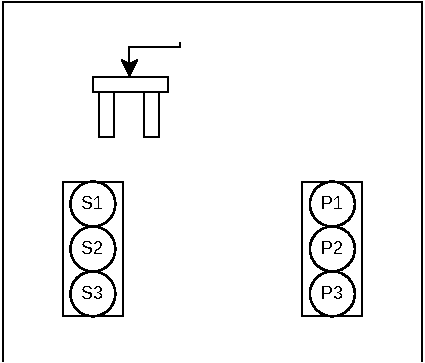
\includegraphics[scale=0.6]{sozai/2.pdf}
  \caption{実験環境(実験1)}
\end{figure}

\subsection{ダイレクトティーチング実験}

\subsubsection{実験手順}
実験は次の手順で行う.

\begin{enumerate}
  \item[(1)] 空圧駆動型ロボットグリッパの電磁弁を操作し,ホワイトボードマーカーを把持させる.
  \item[(2)] マニピュレータを初期位置姿勢付近に移動させる.
  \item[(3)] マニピュレータ制御用ソフトウェアからダイレクトティーチングを実行する.
  \item[(4)] 初期姿勢からS1上部に移動する.
  \item[(5)] S1とP1の中間地点で,ホワイトボードマーカーを3回振る.
  \item[(6)] P1の挿入口にホワイトボードマーカーを指す.
  \item[(7)] マニピュレータを初期位置姿勢付近に戻し,ダイレクトティーチングを終了する.
  \item[(8)] 記録した動作をプレイバックする.プレイバックの様子は動画撮影する.
  \item[(9)] P2とS2,P3とS3の組み合わせでもダイレクトティーチングを実行する.ただし,実行する人を交代させる(全員1度は実行すること(重複してもよい)).実行中の様子を適宜写真,動画撮影し,ティーチングに苦労している点および改善すべき点などを観察する.撮影した写真は考察などに利用する.利用する場合は図として載せること.
\end{enumerate}

\subsubsection{実験結果}
ダイレクトティーチングの実行結果について説明する.
図4.3にダイレクトティーチングのプレイバックの様子を示す.

\subsubsection{考察}
次に,実行結果について考察する.

\subsection{オンラインティーチング実験}

\subsubsection{実験手順}
マニピュレータ制御用ソフトウェアを用いて,オンラインティーチングを行う.
オンラインティーチングはビジュアルプログラミングモードを用いて行う.実験は次の手順で行う.

\begin{enumerate}
  \item[(1)] マニピュレータを初期位置姿勢に移動させる.
  \item[(2)] マニピュレータ制御用ソフトウェアからオンラインティーチングを実行する.
  \item[(3)] 初期姿勢からS1に移動し,ホワイトボードマーカーを把持する動作を行う.その後,ホワイトボードマーカーをS1から抜く.
  \item[(4)] S1とP1の中間地点で,ホワイトボードマーカーを3回振る.なお,マーカーを振る動作のティーチングは最初の1名が行い,その後はティーチングのデータを複製して使用してよい.
  \item[(5)] P1の挿入口にホワイトボードマーカーを指す.
  \item[(6)] マニピュレータを初期位置姿勢に戻す.
  \item[(7)] P2とS2,P3とS3の組み合わせでも同様にティーチングを行う.ただし,実行する人を交代すること.そして,全員1度は実行すること.人数が4人以上いる場合は,挿入口をP1,P2のホワイトボードマーカーをS1,S2にそれぞれ異なる動作にする.実行中の様子を適宜撮影し,ティーチングに苦労している点などを観察する.撮影した写真は考察などに利用する.利用する場合は図として載せること.
  \item[(8)] オンラインティーチングを終了する.
  \item[(9)] 記録した動作をプレイバックする.プレイバックの様子は動画撮影する.
\end{enumerate}

\subsubsection{実験結果および考察}
オンラインティーチングの実行結果について説明する.
図??にダイレクトティーチングのプレイバックの様子を示す.

\subsubsection{考察}
次に,実行結果を考察する.


\section{実験1-2:運動学(3自由度)実験}

\subsection{実験概要}
本実験では,制御PC内で実行されている運動学をエクセルを用いて計算する.
そして,指定された手先位置にマニピュレータを移動させる実験を行う.
マニピュレータは第4~第6関節が0[deg]に固定された3自由度マニピュレータとして扱う.
マニピュレータへの動作入力は関節角度の数値指定によるオンラインティーチングを用いる.

また,図5.1に示すように本実験における逆運動学は目標位置においてのみ計算し,
実験1-2とは異なり途中経路では計算を行わないものとする.

\begin{figure}[h]
  \centering
  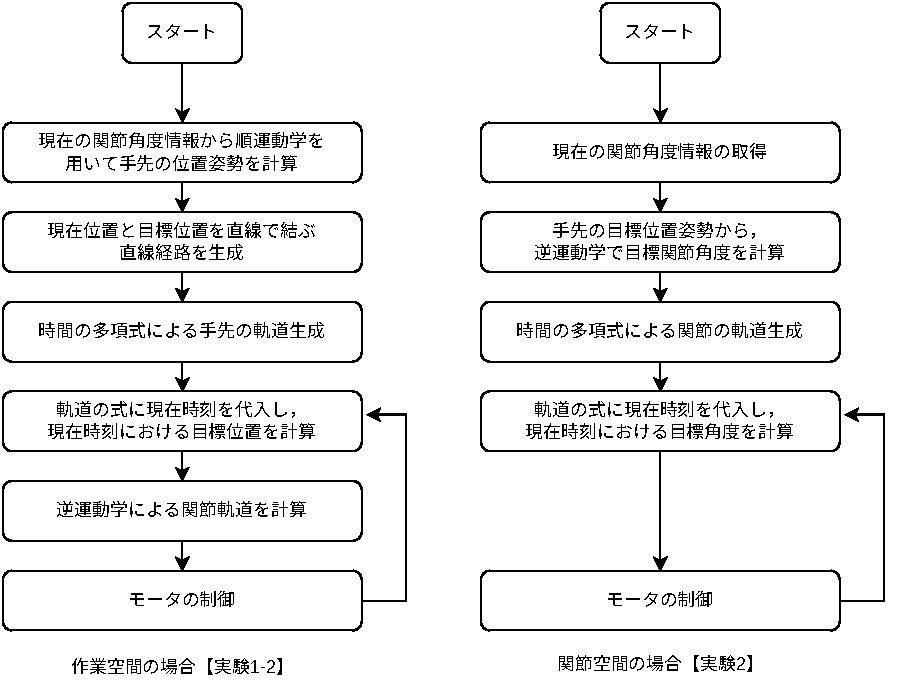
\includegraphics[scale=0.75]{sozai/3.pdf}
  \caption{フローチャート}
\end{figure}

\newpage

\subsection{実験手順}
実験は以下の手順で行う.

\begin{enumerate}
  \item[(1)] 逆運動学(式(2.6),式(2.12)~式(2.14))を計算するエクセルファイルを作成し,表5.2に記された手先位置から関節角度を計算する.数値は小数点第1位まで表記するものとする.
  \item[(2)] 初期位置,No.1~3,初期位置の順に手先位置が到達するようにオンラインティーチングを実行する.
  \item[(3)] 記録した動作をプレイバックする.プレイバックの様子は撮影する.
\end{enumerate}

\begin{table}[h]
  \centering
  \caption{手先位置}
  \begin{tabular}{|c|c|c|c|}
    \hline
    Position No. & $x$ [mm] & $y$ [mm] & $z$ [mm] \\ \hline
    \hline
    1            & 168.1    & 168.1    & 368.8    \\ \hline
    2            & 210.6    & 210.6    & 196.1    \\ \hline
    3            & 541.3    & 0        & 182.8    \\ \hline
  \end{tabular}
\end{table}


\subsection{実験結果}
表5.3に逆運動学の計算結果を示す.また,図5.2に,手先位置がPosition No.2からNo.3に移動した際の経路の模式図を示す.

\begin{table}[h]
  \centering
  \caption{各関節角度の計算結果}
  \begin{tabular}{|c|c|c|c|}
    \hline
    Position No. & $\theta_1$ [deg] & $\theta_2$ [deg] & $\theta_3$ [deg] \\ \hline
    \hline
    1            &                  &                  &                  \\ \hline
    2            &                  &                  &                  \\ \hline
    3            &                  &                  &                  \\ \hline
  \end{tabular}
\end{table}

\subsection{考察}
次に,実行結果の考察を述べる.
